\documentclass[a4paper,10pt]{article}
\usepackage[utf8]{inputenc}
\usepackage[russian]{babel}
\usepackage[T2A, T1]{fontenc}
\usepackage{geometry}
\usepackage{graphicx}

\graphicspath{ {./images/} }
\geometry {
    a4paper,
    left=30mm,
    right=20mm,
    top=10mm,
    bottom=20mm
}

\title{}
\author{}
\date{}

\pdfinfo{%
  /Title    ()
  /Author   ()
  /Creator  ()
  /Producer ()
  /Subject  ()
  /Keywords ()
}

\begin{document}
\begin{titlepage}

\fontsize{14pt}{14pt}\selectfont
\begin{center}
Министерство~науки~и~высшего~образования~Российской~Федерации
Федеральное~государственное~автономное~образовательное~учреждение~высшего~образования\\
«Национальный~исследовательский~университет~ИТМО»\\
\vspace{5mm}
Факультет программной инженерии и компьютерной техники

\vspace{9cm}

\textbf{Лабораторная работа № 6} \\
\vspace{5mm}
``Работа с системой компьютерной вёрстки \TeX''\\
\vspace{5mm}
Вариант № 44

\vfill
\end{center}

\raggedleft
\underline{Выполнил:}\\
Сандов Кирилл Алексеевич\\
\underline{Группа:}\\
P3113\\
\underline{Проверил:}\\
к.т.н. преподаватель Белозубов Александр Владимирович

\vfill
\begin{center}
Санкт-Петербург\\
2022
\end{center}

\thispagestyle{empty}

\end{titlepage}

\setcounter{page}{3}

\fontsize{14pt}{14pt}\selectfont
\section*{\fontsize{16pt}{16pt}\selectfont \centering{Задание}}
\underline{Обязательное задание:}
\parСверстать страницу, максимально похожую на выбранную страницу
из журнала «Квант».

\vspace{3mm}
\noindent\underline{Необязательное задание № 1:}

1. Сверстать титульный лист.

2. Создать файл \verb|main.tex|, в котором будет содержаться преамбула и
ссылки на 2 документа: титульный лист и статью (ссылки создаются с
помощью команды \verb|\input|).

\newpage
\section*{\fontsize{16pt}{16pt}\selectfont \centering{Выбранные страницы из журнала <<Квант>>}}
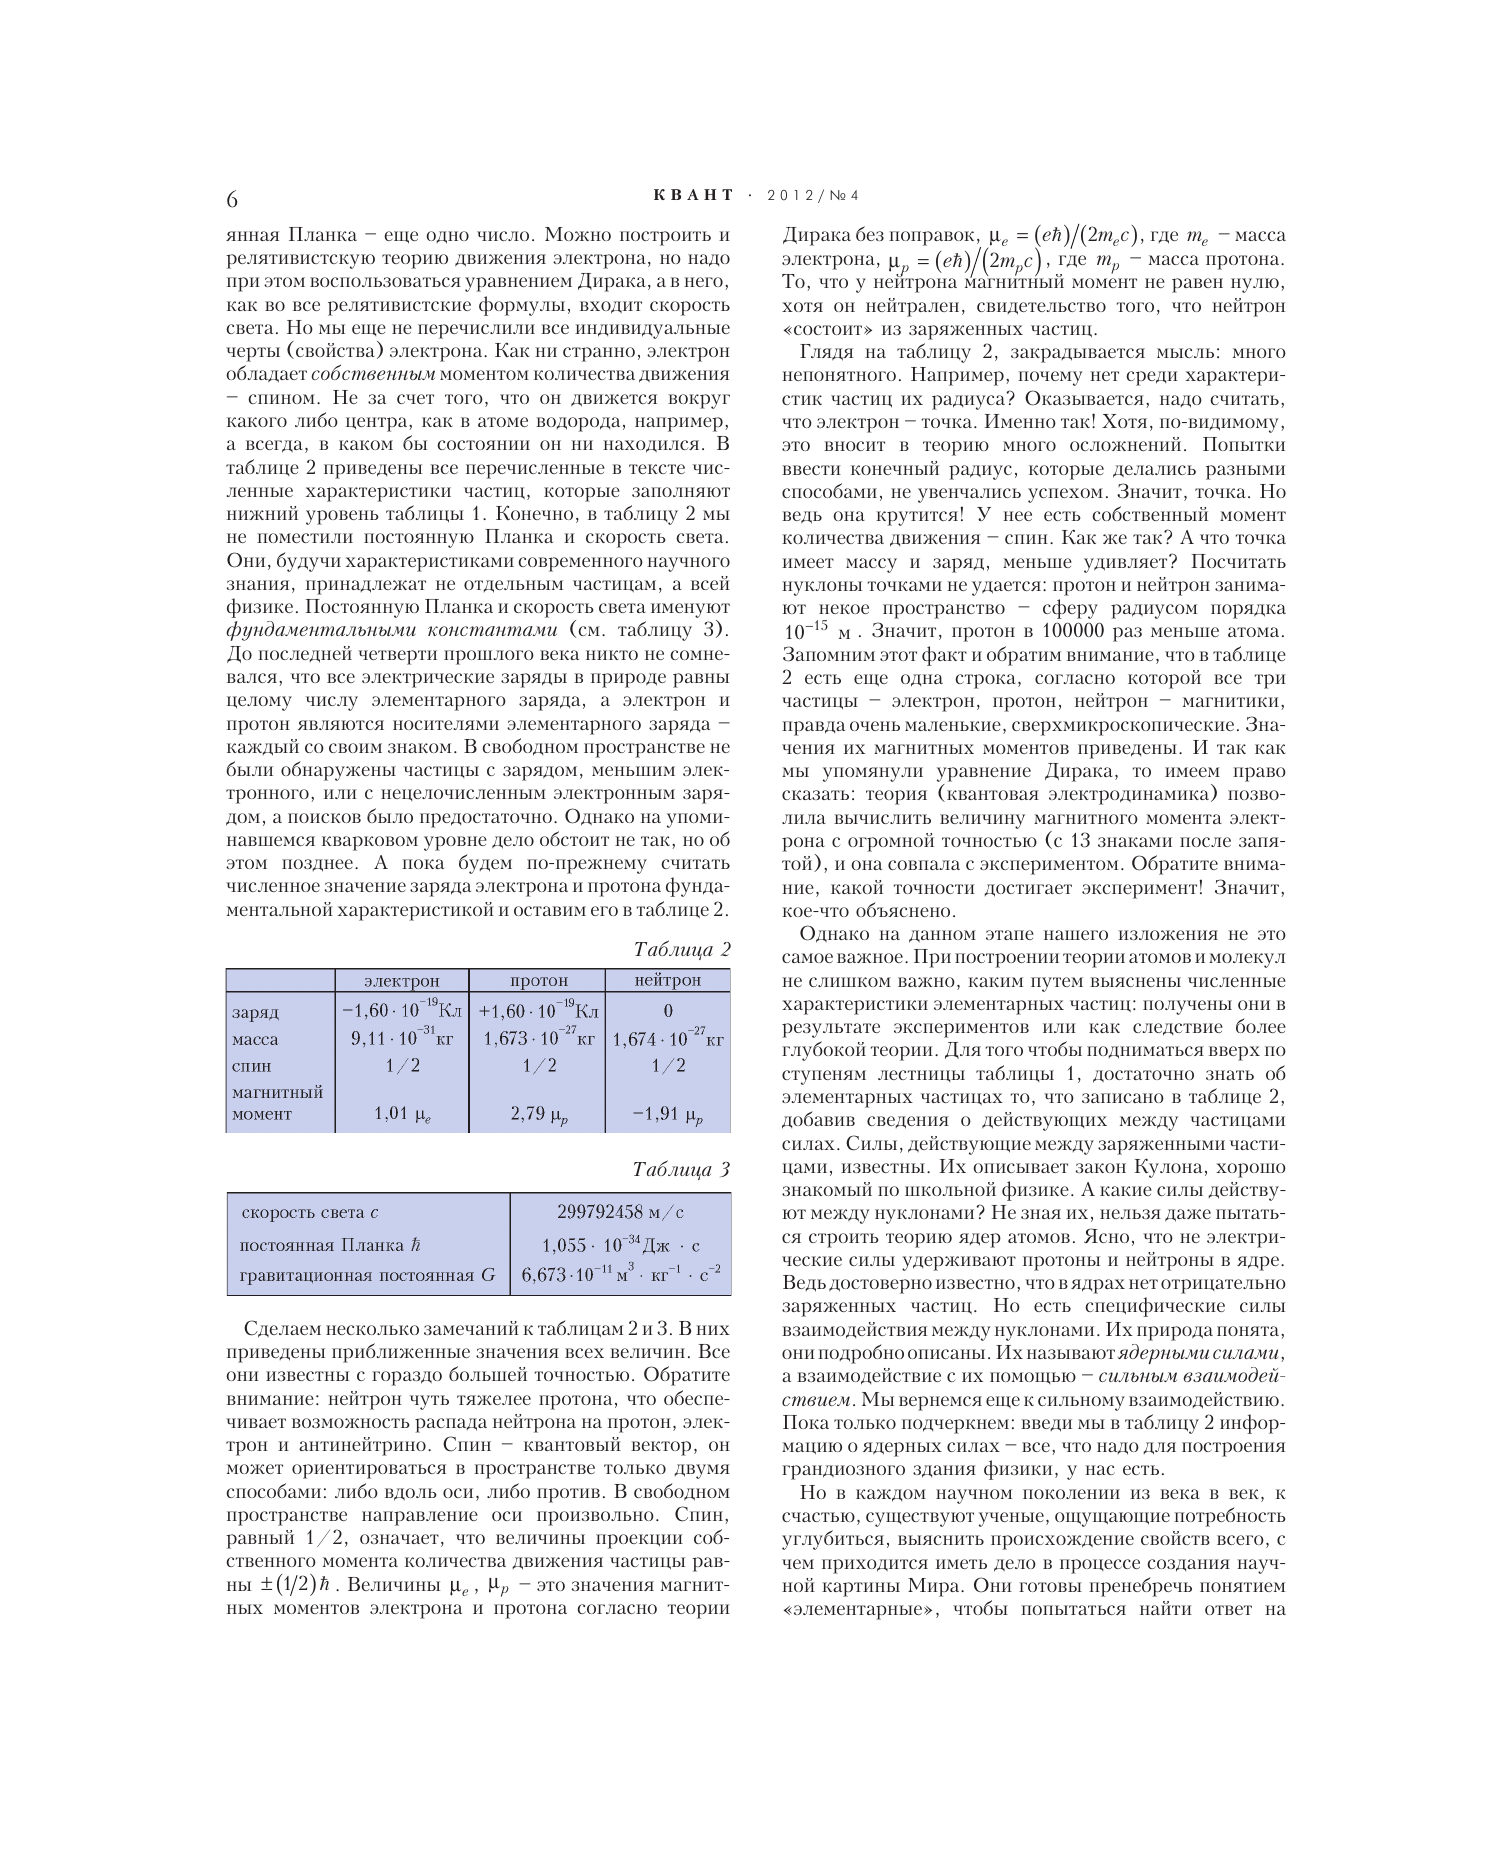
\includegraphics[width=17cm]{page1}
\newpage
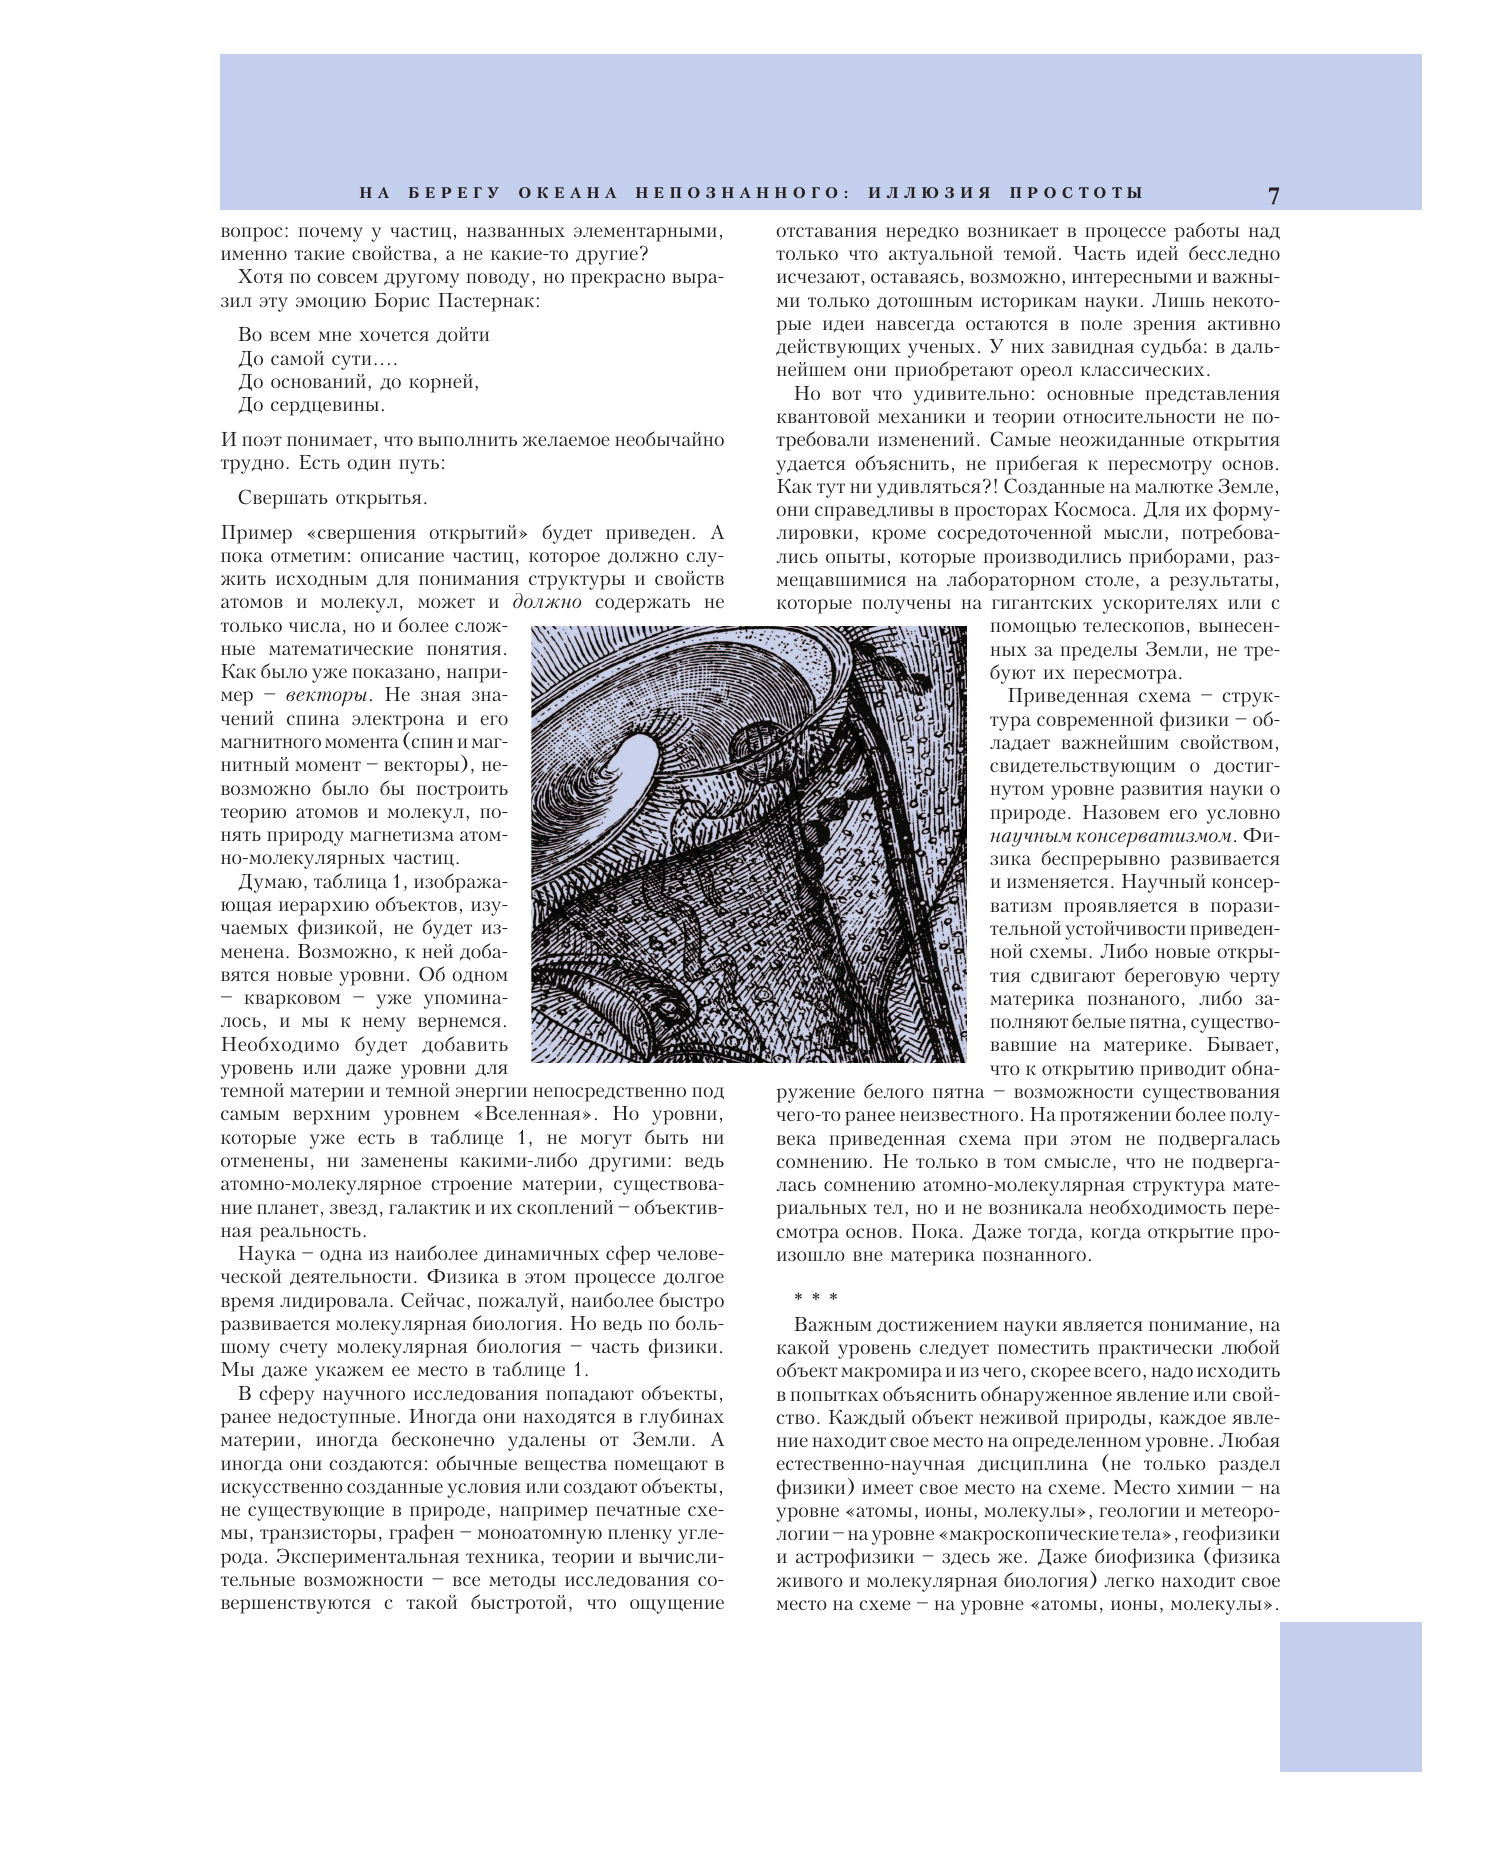
\includegraphics[width=17cm]{page2}

\newpage
\section*{\fontsize{16pt}{16pt}\selectfont \centering{Исходные коды}}
\underline{Обязательное задание:}

\vspace{5mm}
\noindent\verb|article-fragment.tex|
\fontsize{8pt}{8pt}\selectfont
\begin{verbatim}
\fancyhead{} % clear all header fields
\fancyhead[LE]{6} % TODO: page numbers
\fancyhead[CE]{\fontsize{6pt}{5pt}\selectfont \textbf{К В А Н Т} $\cdot$ \textsf{2012 / No 4}}
\fancyhead[RO]{\makebox[\dimexpr\linewidth-3\fboxsep][r]{
7
}
}
\fancyhead[CO]{\colorbox{tableColor}{
\makebox[\dimexpr\linewidth-7\fboxsep][c]{
\fontsize{4pt}{4pt}\selectfont
\textbf{Н\!\;А\quadБ\!\;Е\!\;Р\!\;Е\!\;Г\!\;У\quadО\!\;К\!\;Е\!\;А\!\;Н\!\;А\quadН\!\;Е\!\;П\!
\;О\!\;З\!\;Н\!\;А\!\;Н\!\;Н\!\;О\!\;Г\!\;О:
И\!\;Л\!\;Л\!\;Ю\!\;З\!\;И\!\;Я\quadП\!\;Р\!\;О\!\;С\!\;Т\!\;О\!\;Т\!\;Ы}
}
}
}
\begin{multicols}{2}
\noindent
\fontsize{9pt}{9pt}\selectfont
янная Планка – еще одно число. Можно построить и
релятивистскую теорию движения электрона, но надо
при этом воспользоваться уравнением Дирака, а в него,
как во все релятивистские формулы, входит скорость
света. Но мы еще не перечислили все индивидуальные
черты (свойства) электрона. Как ни странно, электрон
обладает \textit{собственным} моментом количества движения
– спином. Не за счет того, что он движется вокруг
какого либо центра, как в атоме водорода, например,
а всегда, в каком бы состоянии он ни находился. В
таблице \ref{tab:Table2} приведены все перечисленные в тексте численные характеристики частиц,
которые заполняют
нижний уровень таблицы 1. Конечно, в таблицу \ref{tab:Table2} мы
не поместили постоянную Планка и скорость света.
Они, будучи характеристиками современного научного
знания, принадлежат не отдельным частицам, а всей
физике. Постоянную Планка и скорость света именуют
\textit{фундаментальными константами} (см. таблицу \ref{tab:Table3}).
До последней четверти прошлого века никто не сомневался, что все электрические заряды в
природе равны
целому числу элементарного заряда, а электрон и
протон являются носителями элементарного заряда –
каждый со своим знаком. В свободном пространстве не
были обнаружены частицы с зарядом, меньшим электронного, или с нецелочисленным электронным
зарядом, а поисков было предостаточно. Однако на упоминавшемся кварковом уровне дело обстоит
не так, но об
этом позднее. А пока будем по-прежнему считать
численное значение заряда электрона и протона фундаментальной характеристикой и оставим его в
таблице \ref{tab:Table2}.
\begin{center} % table 2
\captionof{table}{}
\label{tab:Table2}
\resizebox{\columnwidth}{!}{
\begin{tblr}{
rows={0, f},
colspec={|p{15mm}|c|c|c|}
}
4
\hline
\SetRow{tableColor}
& электрон & протон & нейтрон \\
\hline
\SetRow{tableColor}
заряд & $-1,60\cdot10^{-19}$Кл & $+1,60\cdot10^{-19}$Кл & 0 \\
\SetRow{tableColor}
масса & $9,11\cdot10^{-31}$кг & $1,673\cdot10^{-27}$кг & $1,674\cdot10^{-27}$кг \\
\SetRow{tableColor}
спин & 1/2 & 1/2 & 1/2 \\
\SetRow{tableColor}
магнитный момент & {$1,01\>\mu_e$} & $2,79\>\mu_p$& $-1,91\>\mu_p$ \\
\hline
\end{tblr}
}
\end{center}
\begin{center} % table 3
\captionof{table}{}
\label{tab:Table3}
\resizebox{\columnwidth}{!}{
\begin{tblr}{
rows={0, f},
colspec={|l|c|}
}
\hline
\SetRow{tableColor}
скорость света $c$ & 299792458 м/c \\
\SetRow{tableColor}
постоянная Планка $\hbar$ & $1,055\cdot10^{-34}Дж\cdotс$ \\
\SetRow{tableColor}
гравитационная постоянная $G$ & $6,673\cdot10^{-11}$м$^{3}\cdot$кг$^{-1}\cdot$с$^{-2}$ \\
\hline
\end{tblr}
}
\end{center}
\par
Сделаем несколько замечаний к таблицам \ref{tab:Table2} и \ref{tab:Table3}. В них
приведены приближенные значения всех величин. Все
они известны с гораздо большей точностью. Обратите
внимание: нейтрон чуть тяжелее протона, что обеспечивает возможность распада нейтрона на
протон, электрон и антинейтрино. Спин – квантовый вектор, он
может ориентироваться в пространстве только двумя
способами: либо вдоль оси, либо против. В свободном
пространстве направление оси произвольно. Спин,
равный 1/2, означает, что величины проекции собственного момента количества движения частицы
равны
$\pm(1/2)\hbar$\>. Величины $\mu_e$, $\mu_p$ – это значения магнитных моментов электрона и
протона согласно теории Дирака без поправок, $\mu_e=(e\hbar)/(2m_ec)$, где $m_e$ – масса
электрона, $\mu_p=(e\hbar)/(2m_pc)$, где – $m_p$ – масса протона.
То, что у нейтрона магнитный момент не равен нулю,
хотя он нейтрален, свидетельство того, что нейтрон
«состоит» из заряженных частиц.
\par
Глядя на таблицу \ref{tab:Table2}, закрадывается мысль: много
непонятного. Например, почему нет среди характеристик частиц их радиуса? Оказывается, надо
считать,
что электрон – точка. Именно так! Хотя, по-видимому,
это вносит в теорию много осложнений. Попытки
ввести конечный радиус, которые делались разными
способами, не увенчались успехом. Значит, точка. Но
ведь она крутится! У нее есть собственный момент
количества движения – спин. Как же так? А что точка
имеет массу и заряд, меньше удивляет? Посчитать
нуклоны точками не удается: протон и нейтрон занимают некое пространство – сферу радиусом
порядка $10^{-15}$ м. Значит, протон в 100000 раз меньше атома.
Запомним этот факт и обратим внимание, что в таблице
\ref{tab:Table2} есть еще одна строка, согласно которой все три
частицы – электрон, протон, нейтрон – магнитики,
правда очень маленькие, сверхмикроскопические. Значения их магнитных моментов приведены. И так
как
мы упомянули уравнение Дирака, то имеем право
сказать: теория (квантовая электродинамика) позволила вычислить величину магнитного момента
электрона с огромной точностью (с 13 знаками после запятой), и она совпала с экспериментом.
Обратите внимание, какой точности достигает эксперимент! Значит,
кое-что объяснено.
\par
Однако на данном этапе нашего изложения не это
самое важное. При построении теории атомов и молекул
не слишком важно, каким путем выяснены численные
характеристики элементарных частиц: получены они в
результате экспериментов или как следствие более
глубокой теории. Для того чтобы подниматься вверх по
ступеням лестницы таблицы 1, достаточно знать об
элементарных частицах то, что записано в таблице \ref{tab:Table2},
добавив сведения о действующих между частицами
силах. Силы, действующие между заряженными частицами, известны. Их описывает закон Кулона,
хорошо
знакомый по школьной физике. А какие силы действуют между нуклонами? Не зная их, нельзя даже
пытаться строить теорию ядер атомов. Ясно, что не электрические силы удерживают протоны и
нейтроны в ядре.
Ведь достоверно известно, что в ядрах нет отрицательно
заряженных частиц. Но есть специфические силы
взаимодействия между нуклонами. Их природа понята,
они подробно описаны. Их называют \textit{ядерными силами},
а взаимодействие с их помощью – \textit{сильным взаимодействием}. Мы вернемся еще к сильному
взаимодействию.
Пока только подчеркнем: введи мы в таблицу \ref{tab:Table2} информацию о ядерных силах – все,
что надо для построения
грандиозного здания физики, у нас есть.
\par
Но в каждом научном поколении из века в век, к
счастью, существуют ученые, ощущающие потребность
углубиться, выяснить происхождение свойств всего, с
чем приходится иметь дело в процессе создания научной картины Мира. Они готовы пренебречь
понятием
«элементарные», чтобы попытаться найти ответ на
вопрос: почему у частиц, названных элементарными,
именно такие свойства, а не какие-то другие?
\par
Хотя по совсем другому поводу, но прекрасно выразил эту эмоцию Борис Пастернак:
\\
\par Во всем мне хочется дойти
\par До самой сути....
\par До оснований, до корней,
\par До сердцевины. \\
\\
И поэт понимает, что выполнить желаемое необычайно
трудно. Есть один путь:
\\
\par Свершать открытья. \\
\\
Пример «свершения открытий» будет приведен. А
пока отметим: описание частиц, которое должно служить исходным для понимания структуры и
свойств
атомов и молекул, может и \textit{должно} содержать не только числа, но и
\parshape 22
0pt \columnwidth% 1
0pt 0.58\columnwidth% 2
0pt 0.58\columnwidth% 3
0pt 0.58\columnwidth% 4
0pt 0.58\columnwidth% 5
0pt 0.58\columnwidth% 6
0pt 0.58\columnwidth% 7
0pt 0.58\columnwidth% 8
0pt 0.58\columnwidth% 9
0pt 0.58\columnwidth% 10
0pt 0.58\columnwidth% 11
0pt 0.58\columnwidth% 12
0pt 0.58\columnwidth% 13
0pt 0.58\columnwidth% 14
0pt 0.58\columnwidth% 15
0pt 0.58\columnwidth% 16
0pt 0.58\columnwidth% 17
0pt 0.58\columnwidth% 18
0pt 0.58\columnwidth% 19
0pt 0.58\columnwidth% 20
0pt 0.58\columnwidth% 21
0pt \columnwidth% 22
\rlap{% Remove horizontal width
\smash{% Remove vertical height
\hspace{\dimexpr\columnwidth+.5\columnsep}% Push content to middle of page
\makebox[0pt][c]{% Centre image in middle of page
% Drop image full height and scale to 12 lines high
\raisebox{-\height}{\includegraphics[height=19\baselineskip]{deco}}%
}%
}%
}\hfill%
\\[-2\baselineskip]
более сложные математические понятия.
Как было уже показано, например – \textit{векторы}. Не зная значений спина электрона и его
магнитного момента (спин и магнитный момент – векторы), невозможно было бы построить
теорию атомов и молекул, понять природу магнетизма атомно-молекулярных частиц.
Думаю, таблица 1, изображающая иерархию объектов, изучаемых физикой, не будет изменена.
Возможно, к ней добавятся новые уровни. Об одном
– кварковом – уже упоминалось, и мы к нему вернемся.
Необходимо будет добавить
уровень или даже уровни для
темной материи и темной энергии непосредственно под
самым верхним уровнем «Вселенная». Но уровни,
которые уже есть в таблице 1, не могут быть ни
отменены, ни заменены какими-либо другими: ведь
атомно-молекулярное строение материи, существование планет, звезд, галактик и их скоплений –
объективная реальность.
Наука – одна из наиболее динамичных сфер человеческой деятельности. Физика в этом процессе
долгое
время лидировала. Сейчас, пожалуй, наиболее быстро
развивается молекулярная биология. Но ведь по большому счету молекулярная биология – часть
физики.
Мы даже укажем ее место в таблице 1.
В сферу научного исследования попадают объекты,
ранее недоступные. Иногда они находятся в глубинах
материи, иногда бесконечно удалены от Земли. А
иногда они создаются: обычные вещества помещают в
искусственно созданные условия или создают объекты,
не существующие в природе, например печатные схемы, транзисторы, графен – моноатомную пленку
углерода. Экспериментальная техника, теории и вычислительные возможности – все методы
исследования совершенствуются с такой быстротой, что ощущение
отставания нередко возникает в процессе работы над
только что актуальной темой. Часть идей бесследно
исчезают, оставаясь, возможно, интересными и важными только дотошным историкам науки. Лишь
некоторые идеи навсегда остаются в поле зрения активно
действующих ученых. У них завидная судьба: в дальнейшем они приобретают ореол классических.
Но вот что удивительно: основные представления квантовой механики и теории относительности не
потребовали изменений.
\parshape 22
0pt \columnwidth% 1
0.42\columnwidth 0.58\columnwidth% 2
0.42\columnwidth 0.58\columnwidth% 3
0.42\columnwidth 0.58\columnwidth% 4
0.42\columnwidth 0.58\columnwidth% 5
0.42\columnwidth 0.58\columnwidth% 6
0.42\columnwidth 0.58\columnwidth% 7
0.42\columnwidth 0.58\columnwidth% 8
0.42\columnwidth 0.58\columnwidth% 9
0.42\columnwidth 0.58\columnwidth% 10
0.42\columnwidth 0.58\columnwidth% 11
7
0.42\columnwidth 0.58\columnwidth% 12
0.42\columnwidth 0.58\columnwidth% 13
0.42\columnwidth 0.58\columnwidth% 14
0.42\columnwidth 0.58\columnwidth% 15
0.42\columnwidth 0.58\columnwidth% 16
0.42\columnwidth 0.58\columnwidth% 17
0.42\columnwidth 0.58\columnwidth% 18
0.42\columnwidth 0.58\columnwidth% 19
0.42\columnwidth 0.58\columnwidth% 20
0.42\columnwidth 0.58\columnwidth% 21
0pt \columnwidth% 22
\noindentСамые неожиданные открытия удается объяснить, не прибегая к пересмотру основ.
Как тут ни удивляться?! Созданные на малютке Земле,
они справедливы в просторах Космоса. Для их формулировки, кроме сосредоточенной мысли,
потребовались опыты, которые производились приборами, размещавшимися на лабораторном столе, а
результаты,
которые получены на гигантских ускорителях или с
помощью телескопов, вынесенных за пределы Земли, не требуют их пересмотра.
Приведенная схема – структура современной физики – обладает важнейшим свойством,
свидетельствующим о достигнутом уровне развития науки о
природе. Назовем его условно
\textit{научным консерватизмом}. Физика беспрерывно развивается
и изменяется. Научный консерватизм проявляется в поразительной устойчивости приведенной схемы.
Либо новые открытия сдвигают береговую черту
материка познаного, либо заполняют белые пятна, существовавшие на материке. Бывает,
что к открытию приводит обнаружение белого пятна – возможности существования
чего-то ранее неизвестного. На протяжении более полувека приведенная схема при этом не
подвергалась
сомнению. Не только в том смысле, что не подвергалась сомнению атомно-молекулярная структура
материальных тел, но и не возникала необходимость пересмотра основ. Пока. Даже тогда, когда
открытие произошло вне материка познанного.
\end{multicols}
\end{verbatim}

\fontsize{14pt}{14pt}\selectfont
\noindent\underline{Необязательное задание:}

\noindent\verb|title.tex|
\fontsize{8pt}{8pt}\selectfont
\begin{verbatim}
\begin{titlepage}
\fontsize{14pt}{14pt}\selectfont
\begin{center}
Министерство науки и высшего образования Российской Федерации
Федеральное государственное автономное образовательное учреждение
высшего образования\\
«Национальный исследовательский университет ИТМО»\\
\vspace{5mm}
Факультет Программной инженерии и компьютерной техники
\vspace{9cm}
\textbf{Лабораторная работа No 6} \\
\vspace{5mm}
``Работа с системой компьютерной вёрстки \TeX''\\
\vspace{5mm}
Вариант No 44
\vfill
\end{center}
\raggedleft
\underline{Выполнил:}\\
Сандов Кирилл Алексеевич\\
\underline{Группа:}\\
P3113\\
\underline{Проверил:}\\
к.т.н. преподаватель Белозубов Александр Владимирович
\vfill
\begin{center}
г. Санкт-Петербург\\
2022
\end{center}
\thispagestyle{empty}
\end{titlepage}
\end{verbatim}

\fontsize{14pt}{14pt}\selectfont
\noindent\verb|main.tex|
\fontsize{8pt}{8pt}\selectfont
\begin{verbatim}
\documentclass{book}
\usepackage[english, russian]{babel}
\usepackage[utf8]{inputenc}
\usepackage[T2A,T1]{fontenc}
\usepackage{fancyhdr}
\usepackage{blindtext}
\usepackage{multicol}
\usepackage{tabularray}
\usepackage{geometry}
\usepackage{graphicx}
\usepackage{caption}
\usepackage{xcolor}
\usepackage{wrapfig}
\usepackage{listings}
\geometry{ % configure padding and layout
a4paper,
left=36mm,
top=40mm,
headheight=5.0mm
}
\graphicspath{ {./images/} }
\captionsetup{ % configure captions to the tables and pictures
aboveskip=0.0mm,
belowskip=0.0mm,
font=footnotesize,
justification=raggedleft,
labelfont=it,
singlelinecheck=off
}
\addtocounter{table}{1} % we start from the 2nd table
\definecolor{tableColor}{HTML}{bec5e0} % table color
\pagestyle{fancy} % header styling
\fancyhead{}
\fancyfoot{}
\renewcommand{\headrulewidth}{0.0mm}
\setlength{\headheight}{-1.0mm}
\renewcommand{\headruleskip}{0.0mm}
\setlength{\columnsep}{9.0mm} % 2 cols text styling
\title{}
\author{}
\date{}
\pdfinfo{
/Title
/Author
/Creator/Producer/Subject/Keywords}
()
()
()
()
()
()
\begin{document}
\begin{titlepage}

\fontsize{14pt}{14pt}\selectfont
\begin{center}
Министерство~науки~и~высшего~образования~Российской~Федерации
Федеральное~государственное~автономное~образовательное~учреждение~высшего~образования\\
«Национальный~исследовательский~университет~ИТМО»\\
\vspace{5mm}
Факультет программной инженерии и компьютерной техники

\vspace{9cm}

\textbf{Лабораторная работа № 6} \\
\vspace{5mm}
``Работа с системой компьютерной вёрстки \TeX''\\
\vspace{5mm}
Вариант № 44

\vfill
\end{center}

\raggedleft
\underline{Выполнил:}\\
Сандов Кирилл Алексеевич\\
\underline{Группа:}\\
P3113\\
\underline{Проверил:}\\
к.т.н. преподаватель Белозубов Александр Владимирович

\vfill
\begin{center}
Санкт-Петербург\\
2022
\end{center}

\thispagestyle{empty}

\end{titlepage}

\newpage
\fancyhead{} % clear all header fields
\fancyhead[LE]{6}  % TODO: page numbers
\fancyhead[CE]{\fontsize{6pt}{5pt}\selectfont \textbf{К В А Н Т} $\cdot$ \textsf{2012 / № 4}}
\fancyhead[RO]{\makebox[\dimexpr\linewidth-3\fboxsep][r]{
    7
    }
  }
\fancyhead[CO]{\colorbox{tableColor}{
  \makebox[\dimexpr\linewidth-7\fboxsep][c]{
    \fontsize{4pt}{4pt}\selectfont
    \textbf{Н\!\;А\quadБ\!\;Е\!\;Р\!\;Е\!\;Г\!\;У\quadО\!\;К\!\;Е\!\;А\!\;Н\!\;А\quadН\!\;Е\!\;П\!\;О\!\;З\!\;Н\!\;А\!\;Н\!\;Н\!\;О\!\;Г\!\;О: И\!\;Л\!\;Л\!\;Ю\!\;З\!\;И\!\;Я\quadП\!\;Р\!\;О\!\;С\!\;Т\!\;О\!\;Т\!\;Ы}
    }
  }
}

\begin{multicols}{2}
\noindent
\fontsize{9pt}{9pt}\selectfont
янная Планка – еще одно число. Можно построить и
релятивистскую теорию движения электрона, но надо
при этом воспользоваться уравнением Дирака, а в него,
как во все релятивистские формулы, входит скорость
света. Но мы еще не перечислили все индивидуальные
черты (свойства) электрона. Как ни странно, электрон
обладает \textit{собственным} моментом количества движения
– спином. Не за счет того, что он движется вокруг
какого либо центра, как в атоме водорода, например,
а всегда, в каком бы состоянии он ни находился. В
таблице \ref{tab:Table2} приведены все перечисленные в тексте численные характеристики частиц, которые заполняют
нижний уровень таблицы 1. Конечно, в таблицу \ref{tab:Table2} мы
не поместили постоянную Планка и скорость света.
Они, будучи характеристиками современного научного
знания, принадлежат не отдельным частицам, а всей
физике. Постоянную Планка и скорость света именуют
\textit{фундаментальными константами} (см. таблицу \ref{tab:Table3}).
До последней четверти прошлого века никто не сомневался, что все электрические заряды в природе равны
целому числу элементарного заряда, а электрон и
протон являются носителями элементарного заряда –
каждый со своим знаком. В свободном пространстве не
были обнаружены частицы с зарядом, меньшим электронного, или с нецелочисленным электронным зарядом, а поисков было предостаточно. Однако на упоминавшемся кварковом уровне дело обстоит не так, но об
этом позднее. А пока будем по-прежнему считать
численное значение заряда электрона и протона фундаментальной характеристикой и оставим его в таблице \ref{tab:Table2}.

\begin{center}  % table 2
\captionof{table}{}
\label{tab:Table2}
\resizebox{\columnwidth}{!}{
\begin{tblr}{
  rows={0, f},
  colspec={|p{15mm}|c|c|c|}
}
\hline
\SetRow{tableColor}
& \textcolor{whiteColor}{электрон} & \textcolor{whiteColor}{протон} & \textcolor{whiteColor}{нейтрон} \\
\hline
\SetRow{tableColor}
заряд & $-1,60\cdot10^{-19}$Кл & $+1,60\cdot10^{-19}$Кл & 0 \\
\SetRow{tableColor}
\textcolor{whiteColor}{масса} & \textcolor{whiteColor}{$9,11\cdot10^{-31}$кг} & \textcolor{whiteColor}{$1,673\cdot10^{-27}$кг} & \textcolor{whiteColor}{$1,674\cdot10^{-27}$кг} \\
\SetRow{tableColor}
спин & 1/2 & 1/2 & 1/2 \\
\SetRow{tableColor}
\textcolor{whiteColor}{магнитный момент} & \textcolor{whiteColor}{$1,01\>\mu_e$} & \textcolor{whiteColor}{$2,79\>\mu_p$}& \textcolor{whiteColor}{$-1,91\>\mu_p$} \\
\hline
\end{tblr}
}
\end{center}

\begin{center}  % table 3
\captionof{table}{}
\label{tab:Table3}
\resizebox{\columnwidth}{!}{
\begin{tblr}{
  rows={0, f},
  colspec={|l|c|}
}
\hline
\SetRow{tableColor}
скорость света $c$ & 299792458 м/c \\
\SetRow{tableColor}
постоянная Планка $\hbar$ & $1,055\cdot10^{-34}Дж\cdotс$ \\
\SetRow{tableColor}
гравитационная постоянная $G$ & $6,673\cdot10^{-11}$м$^{3}\cdot$кг$^{-1}\cdot$с$^{-2}$ \\
\hline
\end{tblr}
}
\end{center}

\par
Сделаем несколько замечаний к таблицам \ref{tab:Table2} и \ref{tab:Table3}. В них
приведены приближенные значения всех величин. Все
они известны с гораздо большей точностью. Обратите
внимание: нейтрон чуть тяжелее протона, что обеспечивает возможность распада нейтрона на протон, электрон и антинейтрино. Спин – квантовый вектор, он
может ориентироваться в пространстве только двумя
способами: либо вдоль оси, либо против. В свободном
пространстве направление оси произвольно. Спин,
равный 1/2, означает, что величины проекции собственного момента количества движения частицы равны
$\pm(1/2)\hbar$\>. Величины $\mu_e$, $\mu_p$ – это значения магнитных моментов электрона и протона согласно теории Дирака без поправок, $\mu_e=(e\hbar)/(2m_ec)$, где $m_e$ – масса
электрона, $\mu_p=(e\hbar)/(2m_pc)$, где – $m_p$ – масса протона.
То, что у нейтрона магнитный момент не равен нулю,
хотя он нейтрален, свидетельство того, что нейтрон
«состоит» из заряженных частиц.
\par
Глядя на таблицу \ref{tab:Table2}, закрадывается мысль: много
непонятного. Например, почему нет среди характеристик частиц их радиуса? Оказывается, надо считать,
что электрон – точка. Именно так! Хотя, по-видимому,
это вносит в теорию много осложнений. Попытки
ввести конечный радиус, которые делались разными
способами, не увенчались успехом. Значит, точка. Но
ведь она крутится! У нее есть собственный момент
количества движения – спин. Как же так? А что точка
имеет массу и заряд, меньше удивляет? Посчитать
нуклоны точками не удается: протон и нейтрон занимают некое пространство – сферу радиусом порядка $10^{-15}$ м. Значит, протон в 100000 раз меньше атома.
Запомним этот факт и обратим внимание, что в таблице
\ref{tab:Table2} есть еще одна строка, согласно которой все три
частицы – электрон, протон, нейтрон – магнитики,
правда очень маленькие, сверхмикроскопические. Значения их магнитных моментов приведены. И так как
мы упомянули уравнение Дирака, то имеем право
сказать: теория (квантовая электродинамика) позволила вычислить величину магнитного момента электрона с огромной точностью (с 13 знаками после запятой), и она совпала с экспериментом. Обратите внимание, какой точности достигает эксперимент! Значит,
кое-что объяснено.
\par
Однако на данном этапе нашего изложения не это
самое важное. При построении теории атомов и молекул
не слишком важно, каким путем выяснены численные
характеристики элементарных частиц: получены они в
результате экспериментов или как следствие более
глубокой теории. Для того чтобы подниматься вверх по
ступеням лестницы таблицы 1, достаточно знать об
элементарных частицах то, что записано в таблице \ref{tab:Table2},
добавив сведения о действующих между частицами
силах. Силы, действующие между заряженными частицами, известны. Их описывает закон Кулона, хорошо
знакомый по школьной физике. А какие силы действуют между нуклонами? Не зная их, нельзя даже пытаться строить теорию ядер атомов. Ясно, что не электрические силы удерживают протоны и нейтроны в ядре.
Ведь достоверно известно, что в ядрах нет отрицательно
заряженных частиц. Но есть специфические силы
взаимодействия между нуклонами. Их природа понята,
они подробно описаны. Их называют \textit{ядерными силами},
а взаимодействие с их помощью – \textit{сильным взаимодействием}. Мы вернемся еще к сильному взаимодействию.
Пока только подчеркнем: введи мы в таблицу \ref{tab:Table2} информацию о ядерных силах – все, что надо для построения
грандиозного здания физики, у нас есть.
\par
Но в каждом научном поколении из века в век, к
счастью, существуют ученые, ощущающие потребность
углубиться, выяснить происхождение свойств всего, с
чем приходится иметь дело в процессе создания научной картины Мира. Они готовы пренебречь понятием
«элементарные», чтобы попытаться найти ответ на
вопрос: почему у частиц, названных элементарными,
именно такие свойства, а не какие-то другие?
\par
Хотя по совсем другому поводу, но прекрасно выразил эту эмоцию Борис Пастернак:
\\
\par Во всем мне хочется дойти
\par До самой сути....
\par До оснований, до корней,
\par До сердцевины. \\
\\
И поэт понимает, что выполнить желаемое необычайно
трудно. Есть один путь:
\\
\par Свершать открытья. \\
\\
Пример «свершения открытий» будет приведен. А
пока отметим: описание частиц, которое должно служить исходным для понимания структуры и свойств
атомов и молекул, может и \textit{должно} содержать не только числа, но и

\parshape 22
  0pt \columnwidth% 1
  0pt 0.58\columnwidth% 2
  0pt 0.58\columnwidth% 3
  0pt 0.58\columnwidth% 4
  0pt 0.58\columnwidth% 5
  0pt 0.58\columnwidth% 6
  0pt 0.58\columnwidth% 7
  0pt 0.58\columnwidth% 8
  0pt 0.58\columnwidth% 9
  0pt 0.58\columnwidth% 10
  0pt 0.58\columnwidth% 11
  0pt 0.58\columnwidth% 12
  0pt 0.58\columnwidth% 13
  0pt 0.58\columnwidth% 14
  0pt 0.58\columnwidth% 15
  0pt 0.58\columnwidth% 16
  0pt 0.58\columnwidth% 17
  0pt 0.58\columnwidth% 18
  0pt 0.58\columnwidth% 19
  0pt 0.58\columnwidth% 20
  0pt 0.58\columnwidth% 21
  0pt \columnwidth% 22
\rlap{% Remove horizontal width
  \smash{% Remove vertical height
    \hspace{\dimexpr\columnwidth+.5\columnsep}% Push content to middle of page
    \makebox[0pt][c]{% Centre image in middle of page
      % Drop image full height and scale to 12 lines high
      \raisebox{-\height}{\includegraphics[height=19\baselineskip]{deco}}%
    }%
  }%
}\hfill%
\\[-2\baselineskip]
более сложные математические понятия.
Как было уже показано, например – \textit{векторы}. Не зная значений спина электрона и его
магнитного момента (спин и магнитный момент – векторы), невозможно было бы построить
теорию атомов и молекул, понять природу магнетизма атомно-молекулярных частиц.
Думаю, таблица 1, изображающая иерархию объектов, изучаемых физикой, не будет изменена. Возможно, к ней добавятся новые уровни. Об одном
– кварковом – уже упоминалось, и мы к нему вернемся.
Необходимо будет добавить
уровень или даже уровни для
темной материи и темной энергии непосредственно под
самым верхним уровнем «Вселенная». Но уровни,
которые уже есть в таблице 1, не могут быть ни
отменены, ни заменены какими-либо другими: ведь
атомно-молекулярное строение материи, существование планет, звезд, галактик и их скоплений – объективная реальность.
Наука – одна из наиболее динамичных сфер человеческой деятельности. Физика в этом процессе долгое
время лидировала. Сейчас, пожалуй, наиболее быстро
развивается молекулярная биология. Но ведь по большому счету молекулярная биология – часть физики.
Мы даже укажем ее место в таблице 1.
В сферу научного исследования попадают объекты,
ранее недоступные. Иногда они находятся в глубинах
материи, иногда бесконечно удалены от Земли. А
иногда они создаются: обычные вещества помещают в
искусственно созданные условия или создают объекты,
не существующие в природе, например печатные схемы, транзисторы, графен – моноатомную пленку углерода. Экспериментальная техника, теории и вычислительные возможности – все методы исследования совершенствуются с такой быстротой, что ощущение
отставания нередко возникает в процессе работы над
только что актуальной темой. Часть идей бесследно
исчезают, оставаясь, возможно, интересными и важными только дотошным историкам науки. Лишь некоторые идеи навсегда остаются в поле зрения активно
действующих ученых. У них завидная судьба: в дальнейшем они приобретают ореол классических.
Но вот что удивительно: основные представления квантовой механики и теории относительности не потребовали изменений.

\parshape 22
  0pt \columnwidth% 1
  0.42\columnwidth 0.58\columnwidth% 2
  0.42\columnwidth 0.58\columnwidth% 3
  0.42\columnwidth 0.58\columnwidth% 4
  0.42\columnwidth 0.58\columnwidth% 5
  0.42\columnwidth 0.58\columnwidth% 6
  0.42\columnwidth 0.58\columnwidth% 7
  0.42\columnwidth 0.58\columnwidth% 8
  0.42\columnwidth 0.58\columnwidth% 9
  0.42\columnwidth 0.58\columnwidth% 10
  0.42\columnwidth 0.58\columnwidth% 11
  0.42\columnwidth 0.58\columnwidth% 12
  0.42\columnwidth 0.58\columnwidth% 13
  0.42\columnwidth 0.58\columnwidth% 14
  0.42\columnwidth 0.58\columnwidth% 15
  0.42\columnwidth 0.58\columnwidth% 16
  0.42\columnwidth 0.58\columnwidth% 17
  0.42\columnwidth 0.58\columnwidth% 18
  0.42\columnwidth 0.58\columnwidth% 19
  0.42\columnwidth 0.58\columnwidth% 20
  0.42\columnwidth 0.58\columnwidth% 21
  0pt \columnwidth% 22
\noindentСамые неожиданные открытия удается объяснить, не прибегая к пересмотру основ.
Как тут ни удивляться?! Созданные на малютке Земле,
они справедливы в просторах Космоса. Для их формулировки, кроме сосредоточенной мысли,
потребовались опыты, которые производились приборами, размещавшимися на лабораторном столе, а результаты,
которые получены на гигантских ускорителях или с
помощью телескопов, вынесенных за пределы Земли, не требуют их пересмотра.
Приведенная схема – структура современной физики – обладает важнейшим свойством,
свидетельствующим о достигнутом уровне развития науки о
природе. Назовем его условно
\textit{научным консерватизмом}. Физика беспрерывно развивается
и изменяется. Научный консерватизм проявляется в поразительной устойчивости приведенной схемы. Либо новые открытия сдвигают береговую черту
материка познаного, либо заполняют белые пятна, существовавшие на материке. Бывает,
что к открытию приводит обнаружение белого пятна – возможности существования
чего-то ранее неизвестного. На протяжении более полувека приведенная схема при этом не подвергалась
сомнению. Не только в том смысле, что не подвергалась сомнению атомно-молекулярная структура материальных тел, но и не возникала необходимость пересмотра основ. Пока. Даже тогда, когда открытие произошло вне материка познанного.
\end{multicols}

\end{document}
\end{verbatim}

\newpage
\fontsize{14pt}{14pt}\selectfont
\section*{\fontsize{16pt}{16pt}\selectfont \centering{Заключение}}
В результате выполнения данной лабораторной работы была изучена система: \LaTeX, в частности следующие темы:
\begin{itemize}
\item Набор текста и математических формул;
\item Форматирование текста;
\item Вывод содержимого в две колонки;
\item Создание таблиц;
\item Создание изображений и их позиционирование в тексте;
\item Добавление подписей к изображениям и таблицам, а также ссылки на них в тексте;
\item Использование сторонних пакетов для дополнительных возможностей.
\end{itemize}

\newpage
\fontsize{14pt}{14pt}\selectfont
\section*{\fontsize{16pt}{16pt}\selectfont \centering{Список использованных источников}}
\nocite{*}
\bibliographystyle{plain}
\bibliography{texed-report.bib}

\end{document}
